\documentclass[aspectratio=169]{beamer}

% ==== Theme & basic look ====
\usetheme{Madrid}
\usecolortheme{seahorse}
\setbeamertemplate{navigation symbols}{}
\setbeamertemplate{footline}[frame number]


% Packages for mathematics  
\usepackage{amsmath}  
\usepackage{amsfonts}  
\usepackage{amssymb}  
\usepackage{bm}
\usepackage{CJKutf8}
% Support for \Tilde macro used throughout
\providecommand{\Tilde}[1]{\tilde{#1}}
\providecommand{\proofname}{Proof}
\makeatletter
\newenvironment<>{proofs}[1][\proofname]{%
    \par
    \def\insertproofname{#1.}%
    \usebeamertemplate{proof begin}#2}
  {\usebeamertemplate{proof end}}
\makeatother

% Math shorthand and vector symbols
\newcommand{\grad}{\nabla}
\newcommand{\EE}{\mathbb{E}}
\newcommand{\dd}{\mathrm{d}}
\newcommand{\kbT}{k_B T}
\newcommand{\vx}{\mathbf{x}}

% Bold vector/time-indexed variables
\newcommand{\vxz}{\mathbf{x}_0}
\newcommand{\vxt}{\mathbf{x}_t}
\newcommand{\alpt}{\alpha_t}
\newcommand{\sigt}{\sigma_t}
\newcommand{\veps}{\boldsymbol{\epsilon}}
\newcommand{\vF}{\mathbf{F}}

% Title page details:   
\title[AI for Science]{AI for Science: Bridging Machine Learning and Scientific Discovery}  
\author{Pipi Hu}  
\institute[BIMSA]{Beijing Institute of Mathematical Sciences and Applications}  
\date{\today}  

\pgfdeclareimage[width=2cm]{logo}{../figures/logo.png}
\logo{\pgfuseimage{logo}}

% Outline slide (moved to later; avoid frame before \begin{document})

\setbeamertemplate{navigation symbols}{}
\AtBeginSection[]  
{  
    \begin{frame}<beamer>{Outline}         
        \tableofcontents[currentsection]  
    \end{frame}  
}  
  
\AtBeginSubsection[]  
{  
    \begin{frame}<beamer>{Outline}         
        \tableofcontents[currentsection,currentsubsection]  
    \end{frame}  
}  

\begin{document}  
  
% Title slide  
\begin{frame}  
  \titlepage  
\end{frame}  

\begin{frame}{Feynman's words}
\centering
    What I cannot create, I do not understand.
\end{frame}
  
% Presentation slides  

\section{Introduction: AI for Science}

\begin{frame}{What is AI for Science?}
AI for Science represents the intersection of artificial intelligence and scientific research, where machine learning methods are applied to accelerate scientific discovery.
\begin{itemize}
    \item \textcolor{red}{Drug Discovery}: Predicting molecular properties and designing new compounds
    \item \textcolor{red}{Materials Science}: Discovering new materials with desired properties
    \item \textcolor{red}{Climate Modeling}: Understanding and predicting climate patterns
    \item \textcolor{red}{Physics}: Solving complex physical systems and equations
    \item \textcolor{red}{Biology}: Understanding protein folding and biological processes
\end{itemize}
\end{frame}

\begin{frame}{Key Challenges in AI for Science}
Scientific problems present unique challenges for machine learning:
\begin{enumerate}
    \item \textbf{Data scarcity}: Limited experimental data, expensive to collect
    \item \textbf{Physical constraints}: Solutions must obey physical laws
    \item \textbf{Interpretability}: Scientific understanding requires explainable models
    \item \textbf{Uncertainty quantification}: Scientific predictions need confidence bounds
    \item \textbf{Multi-scale phenomena}: From quantum to macroscopic scales
\end{enumerate}
\end{frame}

\section{Physics-Informed Neural Networks (PINNs)}

\begin{frame}{Physics-Informed Neural Networks}
PINNs incorporate physical laws directly into neural network training:
\begin{equation}
    \mathcal{L} = \mathcal{L}_{data} + \lambda \mathcal{L}_{physics}
\end{equation}
where
\begin{itemize}
    \item $\mathcal{L}_{data}$: Standard data fitting loss
    \item $\mathcal{L}_{physics}$: Physics constraint loss (PDEs, conservation laws)
    \item $\lambda$: Weighting parameter balancing data and physics
\end{itemize}
\end{frame}

\begin{frame}{Example: Solving PDEs with PINNs}
Consider the heat equation:
\begin{equation}
    \frac{\partial u}{\partial t} = \alpha \nabla^2 u + f(x,t)
\end{equation}
with boundary conditions $u(x,0) = g(x)$ and $u(\partial\Omega,t) = h(x,t)$.

The physics loss becomes:
\begin{equation}
    \mathcal{L}_{physics} = \left\|\frac{\partial u_{NN}}{\partial t} - \alpha \nabla^2 u_{NN} - f\right\|^2 + \lambda_1 \left\|u_{NN}(x,0) - g(x)\right\|^2 + \lambda_2 \left\|u_{NN}(\partial\Omega,t) - h(x,t)\right\|^2
\end{equation}
where $u_{NN}(x,t;\theta)$ is the neural network approximation.
\end{frame}

\begin{frame}{Advantages of PINNs}
\begin{itemize}
    \item \textbf{No mesh required}: Unlike traditional numerical methods
    \item \textbf{Unified framework}: Handle forward and inverse problems
    \item \textbf{Data fusion}: Combine sparse data with physical knowledge
    \item \textbf{Parameter discovery}: Learn unknown parameters in PDEs
\end{itemize}

\textbf{Challenges:}
\begin{itemize}
    \item Training can be unstable
    \item Requires careful hyperparameter tuning
    \item May struggle with complex geometries
\end{itemize}
\end{frame}

\section{Molecular Property Prediction}

\begin{frame}{Molecular Representation Learning}
Converting molecules to machine-readable formats:
\begin{itemize}
    \item \textbf{SMILES strings}: Text-based molecular representation
    \item \textbf{Graph neural networks}: Molecular graphs with atoms as nodes, bonds as edges
    \item \textbf{3D coordinates}: Spatial arrangement of atoms
    \item \textbf{Descriptors}: Hand-crafted molecular features
\end{itemize}
\end{frame}

\begin{frame}{Graph Neural Networks for Molecules}
For a molecular graph $G = (V, E)$ with atoms $v_i \in V$ and bonds $e_{ij} \in E$:

\textbf{Message passing:}
\begin{equation}
    h_v^{(l+1)} = \text{UPDATE}\left(h_v^{(l)}, \text{AGGREGATE}\left(\{h_u^{(l)} : u \in \mathcal{N}(v)\}\right)\right)
\end{equation}

\textbf{Property prediction:}
\begin{equation}
    y = \text{READOUT}(\{h_v^{(L)} : v \in V\})
\end{equation}
where $L$ is the number of message passing layers.
\end{frame}

\begin{frame}{Applications in Drug Discovery}
\begin{itemize}
    \item \textbf{Property prediction}: Solubility, toxicity, binding affinity
    \item \textbf{Molecular generation}: Designing new drug candidates
    \item \textbf{Retrosynthesis}: Planning synthetic routes
    \item \textbf{Protein-ligand binding}: Predicting drug-target interactions
\end{itemize}

\textbf{Key datasets:}
\begin{itemize}
    \item QM9: 134k small organic molecules; GEOM-Drugs
    \item ChEMBL: Large-scale bioactivity data
    \item PDB: Protein structures; AlphaFoldDB
\end{itemize}
\end{frame}

\section{Climate and Environmental Modeling}

\begin{frame}{Climate Modeling with AI}
Climate systems involve complex interactions across multiple scales:
\begin{equation}
    \frac{\partial \mathbf{u}}{\partial t} + (\mathbf{u} \cdot \nabla)\mathbf{u} = -\frac{1}{\rho}\nabla p + \nu \nabla^2 \mathbf{u} + \mathbf{F}
\end{equation}
where $\mathbf{u}$ is velocity, $p$ is pressure, and $\mathbf{F}$ represents external forces.
\end{frame}

\begin{frame}{Weather Prediction}
\textbf{Traditional approach:} Numerical weather prediction (NWP) using physics-based models.

\textbf{AI approach:} Deep learning models trained on historical weather data:
\begin{itemize}
    \item \textbf{ConvLSTM}: Spatiotemporal weather prediction
    \item \textbf{Graph neural networks}: Modeling atmospheric dynamics
    \item \textbf{Transformer models}: Long-range dependencies in weather patterns; ViT; Swin Transformer;
\end{itemize}

\textbf{Hybrid approach:} Combining AI with traditional NWP for improved accuracy.
\end{frame}

\begin{frame}{Climate Change Detection}
Using AI to detect and attribute climate change:
\begin{itemize}
    \item \textbf{Pattern recognition}: Identifying climate change signatures
    \item \textbf{Attribution studies}: Linking extreme events to climate change
    \item \textbf{Scenario modeling}: Predicting future climate under different emissions
\end{itemize}

\textbf{Key challenges:}
\begin{itemize}
    \item Limited historical data
    \item Non-stationary climate system
    \item Uncertainty quantification
\end{itemize}
\end{frame}

\section{Protein Folding and Structure Prediction}

\begin{frame}{The Protein Folding Problem}
Proteins fold from linear amino acid sequences to 3D structures:
\begin{equation}
    \text{Sequence: } \text{ACDEFGHIKLMNPQRSTVWY} \rightarrow \text{3D Structure}
\end{equation}

\textbf{Key challenges:}
\begin{itemize}
    \item Exponential number of possible conformations
    \item Complex energy landscapes
    \item Multiple timescales (nanoseconds to seconds)
\end{itemize}
\end{frame}

\begin{frame}{AlphaFold and Structure Prediction}
\textbf{AlphaFold approach:}
\begin{enumerate}
    \item \textbf{Multiple sequence alignment}: Evolutionary information
    \item \textbf{Attention mechanisms}: Long-range interactions
    \item \textbf{Structure module}: 3D coordinate prediction
    \item \textbf{Confidence estimation}: Reliability of predictions
\end{enumerate}

\textbf{Key innovations:}
\begin{itemize}
    \item End-to-end differentiable architecture
    \item Integration of evolutionary and physical constraints
    \item Uncertainty quantification
\end{itemize}
\end{frame}

\begin{frame}{architecture}
    \begin{figure}
        \centering
        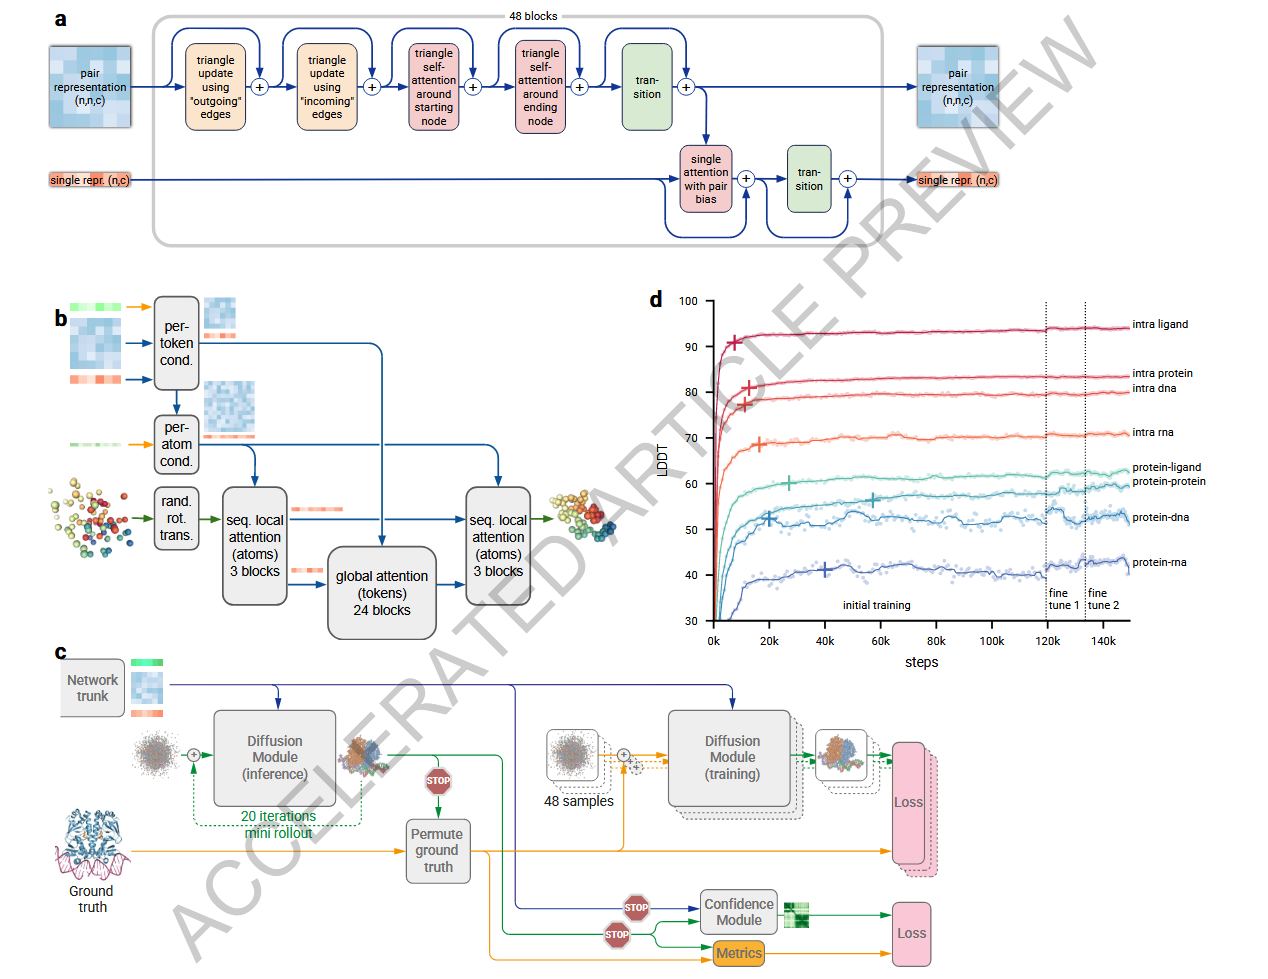
\includegraphics[width=0.5\textwidth]{../figures/alphafold3.png}
        \caption{The architecture of AlphaFold 3.}
    \end{figure}
\end{frame}

\begin{frame}{Impact of AlphaFold}
\begin{itemize}
    \item \textbf{Structural biology revolution}: Millions of protein structures predicted
    \item \textbf{Drug discovery}: Better understanding of drug targets
    \item \textbf{Protein design}: Engineering proteins with desired functions
    \item \textbf{Evolutionary biology}: Understanding protein evolution
\end{itemize}

\textbf{Current limitations:}
\begin{itemize}
    \item Limited accuracy for disordered regions
    \item Challenges with protein complexes
    \item Difficulty with membrane proteins
\end{itemize}
\end{frame}

\section{Materials Discovery}

\begin{frame}{Materials Property Prediction}
Predicting material properties from composition and structure:
\begin{itemize}
    \item \textbf{Electronic properties}: Band gap, conductivity, magnetic properties
    \item \textbf{Mechanical properties}: Elastic modulus, strength, hardness
    \item \textbf{Thermal properties}: Heat capacity, thermal conductivity
    \item \textbf{Optical properties}: Refractive index, absorption spectra
\end{itemize}
\end{frame}

\begin{frame}{Crystal Structure Representation}
\textbf{Periodic systems:} Representing crystal structures with periodic boundary conditions.

\textbf{Graph representations:}
\begin{itemize}
    \item \textbf{Crystal graphs}: Atoms as nodes, bonds as edges
    \item \textbf{Periodic embeddings}: Handling translational symmetry
    \item \textbf{Multi-scale features}: From atomic to macroscopic properties
\end{itemize}

\textbf{Deep learning approaches:}
\begin{itemize}
    \item \textbf{CGCNN}: Crystal Graph Convolutional Neural Networks
    \item \textbf{SchNet}: Quantum-chemical property prediction
    \item \textbf{MEGNet}: Materials property prediction
\end{itemize}
\end{frame}

\begin{frame}{High-Throughput Materials Discovery}
\textbf{Computational screening:}
\begin{enumerate}
    \item Generate candidate materials
    \item Predict properties using ML models
    \item Filter promising candidates
    \item Experimental validation
\end{enumerate}

\textbf{Key databases:}
\begin{itemize}
    \item \textbf{Materials Project}: 150k+ materials with computed properties
    \item \textbf{OQMD}: Open Quantum Materials Database
    \item \textbf{AFLOW}: Automatic Flow for Materials Discovery
\end{itemize}
\end{frame}

\section{Scientific Computing and Simulation}

\begin{frame}{Accelerating Scientific Simulations}
AI can accelerate traditional scientific computing:
\begin{itemize}
    \item \textbf{Surrogate models}: Fast approximations of expensive simulations, fast and efficient such as in nuclear fusion
    \item \textbf{Multiscale modeling}: Bridging different length and time scales
    \item \textbf{Parameter optimization}: Finding optimal simulation parameters
    \item \textbf{Uncertainty quantification}: Propagating uncertainties through simulations
\end{itemize}
\end{frame}

\begin{frame}{Neural Operators}
Learning mappings between function spaces:
\begin{equation}
    G: \mathcal{U} \rightarrow \mathcal{V}, \quad u \mapsto v
\end{equation}
where $\mathcal{U}$ and $\mathcal{V}$ are function spaces.

\textbf{Examples:}
\begin{itemize}
    \item \textbf{Neural ODEs}: Learning dynamics of ordinary differential equations
    \item \textbf{Neural PDEs}: Solving partial differential equations
    \item \textbf{Fourier Neural Operators}: Learning in frequency domain
\end{itemize}
\end{frame}

\begin{frame}{Applications in Scientific Computing}
\begin{itemize}
    \item \textbf{Fluid dynamics}: Turbulence modeling, flow prediction
    \item \textbf{Quantum chemistry}: Electronic structure calculations
    \item \textbf{Solid mechanics}: Stress analysis, fracture prediction
    \item \textbf{Electromagnetics}: Wave propagation, antenna design
\end{itemize}

\textbf{Benefits:}
\begin{itemize}
    \item Orders of magnitude speedup
    \item Reduced computational cost
    \item Real-time predictions
\end{itemize}
\end{frame}

\section{Challenges and Future Directions}

\begin{frame}{Current Challenges in AI for Science}
\begin{enumerate}
    \item \textbf{Data quality and quantity}: Limited, noisy, or biased scientific data
    \item \textbf{Physical consistency}: Ensuring AI predictions obey physical laws
    \item \textbf{Interpretability}: Understanding what AI models learn
    \item \textbf{Generalization}: Models that work across different domains
    \item \textbf{Uncertainty quantification}: Reliable error estimates
\end{enumerate}
\end{frame}

\begin{frame}{Future Directions}
\begin{itemize}
    \item \textbf{Foundation models for science}: Large-scale models trained on scientific data
    \item \textbf{Automated hypothesis generation}: AI systems that propose new scientific theories
    \item \textbf{Scientific reasoning}: AI that can perform logical scientific reasoning
    \item \textbf{Multimodal scientific AI}: Integrating different types of scientific data
    \item \textbf{Scientific collaboration}: AI systems that work alongside human scientists
\end{itemize}
\end{frame}

\begin{frame}{Ethical Considerations}
\begin{itemize}
    \item \textbf{Scientific integrity}: Ensuring AI doesn't introduce bias in scientific research
    \item \textbf{Reproducibility}: Making AI for science research reproducible
    \item \textbf{Open science}: Sharing models, data, and code
    \item \textbf{Scientific communication}: How AI affects scientific publishing and peer review
\end{itemize}
\end{frame}

\section{Selected papers}

\subsection{SimpleFold}
\begin{frame}{Concept \& Setup}
\textbf{Goal.} Predict full-atom 3D structures from an amino-acid sequence using a \emph{general-purpose} Transformer trained with flow matching. \\
\medskip
\textbf{Design stance.}
\begin{itemize}
  \item No MSA, no explicit pair representations, no triangular updates, no equivariant blocks.
  \item Treat sequence as a conditioning signal (like a text prompt) and generate all-atom coordinates.
\end{itemize}
\end{frame}

%----------------------------------------
\begin{frame}{Flow-Matching Scheme}
\textbf{Continuous-time generation.}
\[
\mathrm{d}\bm{x}_t = \bm{v}_\theta(\bm{x}_t,t)\,\mathrm{d}t,\quad t\in[0,1]
\]
Map a tractable prior $p_0$ (Gaussian) to data $p_D$ via a learned velocity field. \\
\medskip
\textbf{Training interpolant (rectified flow).}
\[
\bm{x}_t = t\,\bm{x} + (1-t)\,\bm{\epsilon},\qquad \bm{\epsilon}\sim\mathcal{N}(0,\mathbf{I}),\ \ \bm{x}\sim p_D
\]
\textbf{Target velocity:}\ \  $\bm{v}_t = \bm{x}-\bm{\epsilon}$. \\
\textbf{Loss:}\ \ $\mathbb{E}\big[\lVert \bm{v}_\theta(\bm{x}_t,t)-\bm{v}_t\rVert_2^2\big]$.
\end{frame}

%----------------------------------------
\begin{frame}{Sampling}
\textbf{Stochastic flow sampling.} Initialize $\bm{x}_0\sim\mathcal{N}(0,\mathbf{I})$, integrate to $t=1$ with Euler–Maruyama:
\[
\mathrm{d}\bm{x}_t = \bm{v}_\theta(\bm{x}_t,s,t)\,\mathrm{d}t
+ \tfrac{1}{2}w(t)\,\bm{s}_\theta(\bm{x}_t,s,t)\,\mathrm{d}t
+ \sqrt{\tau\,w(t)}\,\mathrm{d}\bar{\bm{W}}_t,
\]
where $\bm{s}_\theta=\dfrac{t\,\bm{v}_\theta-\bm{x}_t}{1-t}$ and $w(t)=\dfrac{2(1-t)}{t+\eta}$. \\
\textbf{Role of $\tau$.} Controls diversity/accuracy trade-off for ensembles.
\end{frame}

%----------------------------------------
\begin{frame}{Folding with Flow Matching}
\textbf{Conditioning.} Given sequence $s$ and $N_a$ heavy atoms:
\[
\bm{x}_t,\bm{x},\bm{\epsilon}\in\mathbb{R}^{N_a\times 3},\qquad \bm{v}_\theta=\bm{v}_\theta(\bm{x}_t,s,t)
\]
\textbf{Main objective (per-atom average).}
\[
\mathcal{L}_{\text{FM}}=\mathbb{E}_{\bm{x},s,\bm{\epsilon},t}
\left[\tfrac{1}{N_a}\left\lVert \bm{v}_\theta(\bm{x}_t,s,t)-(\bm{x}-\bm{\epsilon})\right\rVert_2^2\right]
\]
\textbf{Structural term (LDDT-inspired).} One-step Euler estimate $\hat{\bm{x}}(\bm{x}_t)=\bm{x}_t+(1-t)\bm{v}_\theta(\bm{x}_t,s,t)$ and penalize local distance errors:
\[
\mathcal{L}_{\text{LDDT}}=\mathbb{E}\!\left[\frac{\sum_{i\neq j}\mathbf{1}(\delta_{ij}\!<\!C)\,\sigma\!\left(\lVert \delta_{ij}-\hat{\delta}^{\,t}_{ij}\rVert\right)}
{\sum_{i\neq j}\mathbf{1}(\delta_{ij}\!<\!C)}\right]
\]
\textbf{Total loss:}\ \ $\mathcal{L}=\mathcal{L}_{\text{FM}}+\alpha(t)\mathcal{L}_{\text{LDDT}}$. \\
\textbf{Timestep resampling.} $p(t)=0.98\,\mathrm{LogisticNormal}(0.8,1.7)+0.02\,\mathcal{U}(0,1)$, biased toward $t\!\to\!1$ for fine details.
\end{frame}

%----------------------------------------
\begin{frame}{Architecture Overview}
\textbf{Three modules, one block type.}
\begin{enumerate}
  \item \textbf{Atom encoder} (local attention): noisy coords $\bm{x}_t$ + atom features $\to$ atom tokens $\bm{a}\in\mathbb{R}^{N_a\times d_a}$.
  \item \textbf{Residue trunk} (heavy): group/pool atom tokens to residue tokens $\bm{r}\in\mathbb{R}^{N_r\times d_a}$, concat with frozen PLM embeddings $e\in\mathbb{R}^{N_r\times d_e}$ from ESM2-3B, process with standard Transformer blocks with adaptive layers.
  \item \textbf{Atom decoder} (local attention): ungroup residue tokens back to atoms, add skip from encoder, predict velocity $\hat{\bm{v}}_t$.
\end{enumerate}
\textbf{Blocks.} QK-normalization, SwiGLU FFN, adaptive scale/shift by $t$; all non-equivariant, no pair/triangle stacks. \\
\textbf{Positional encodings.} RoPE in trunk; 4D axial RoPE in atom modules (3D reference conformer coords + residue index).
\end{frame}

%----------------------------------------
\begin{frame}{Design Choices vs Prior Work}
\begin{itemize}
  \item \textbf{No MSA}, \textbf{no explicit pair representation}, \textbf{no triangular updates}.
  \item Learn SO(3) symmetries via \textbf{data augmentation} rather than equivariance constraints.
  \item Hierarchical compute: \emph{fine} (atoms) $\to$ \emph{coarse} (residues) $\to$ \emph{fine} (atoms). 
  \item Frozen PLM (ESM2-3B) supplies sequence conditioning; folding model is trained end-to-end with flow matching.
\end{itemize}
\end{frame}


%----------------------------------------
\begin{frame}{Confidence Module (pLDDT)}
\textbf{What.} A separate 4-layer Transformer predicts per-residue pLDDT (0–100). \\
\textbf{How.}
\begin{itemize}
  \item Freeze the folding model; feed generated $\hat{\bm{x}}$ with $t{=}1$ to get final residue tokens.
  \item Train pLDDT head with cross-entropy over 50 bins. 
\end{itemize}
\textbf{Use.} Correlates with LDDT-C$\alpha$ and can score structures from other models.
\end{frame}

%----------------------------------------
\begin{frame}{Training Data \& Regime}
\textbf{Data sources.}
\begin{itemize}
  \item PDB (cutoff May 2020) $\sim$160k structures.
  \item AFDB SwissProt subset (pLDDT mean $>$85, std $<$15) $\sim$270k.
  \item AFESM representatives filtered at pLDDT $>$ 0.8 $\sim$1.9M.
  \item For 3B model: extended AFESM-E up to $\sim$8.6M distilled structures (max 10 per cluster, mean pLDDT $>$ 80).
\end{itemize}
\textbf{Training.}
\begin{itemize}
  \item Pre-train at seq length 256; $\alpha(t)=1$; AdamW $1\mathrm{e}{-4}$; EMA 0.999; large effective batch.
  \item Finetune on PDB+SwissProt at seq length 512; $\alpha(t)=1+8\,\mathrm{ReLU}(t-0.5)$ up to 5 near $t{=}1$.
\end{itemize}
\end{frame}

%----------------------------------------
\begin{frame}{Structure and Results}
\begin{figure}
    \centering
    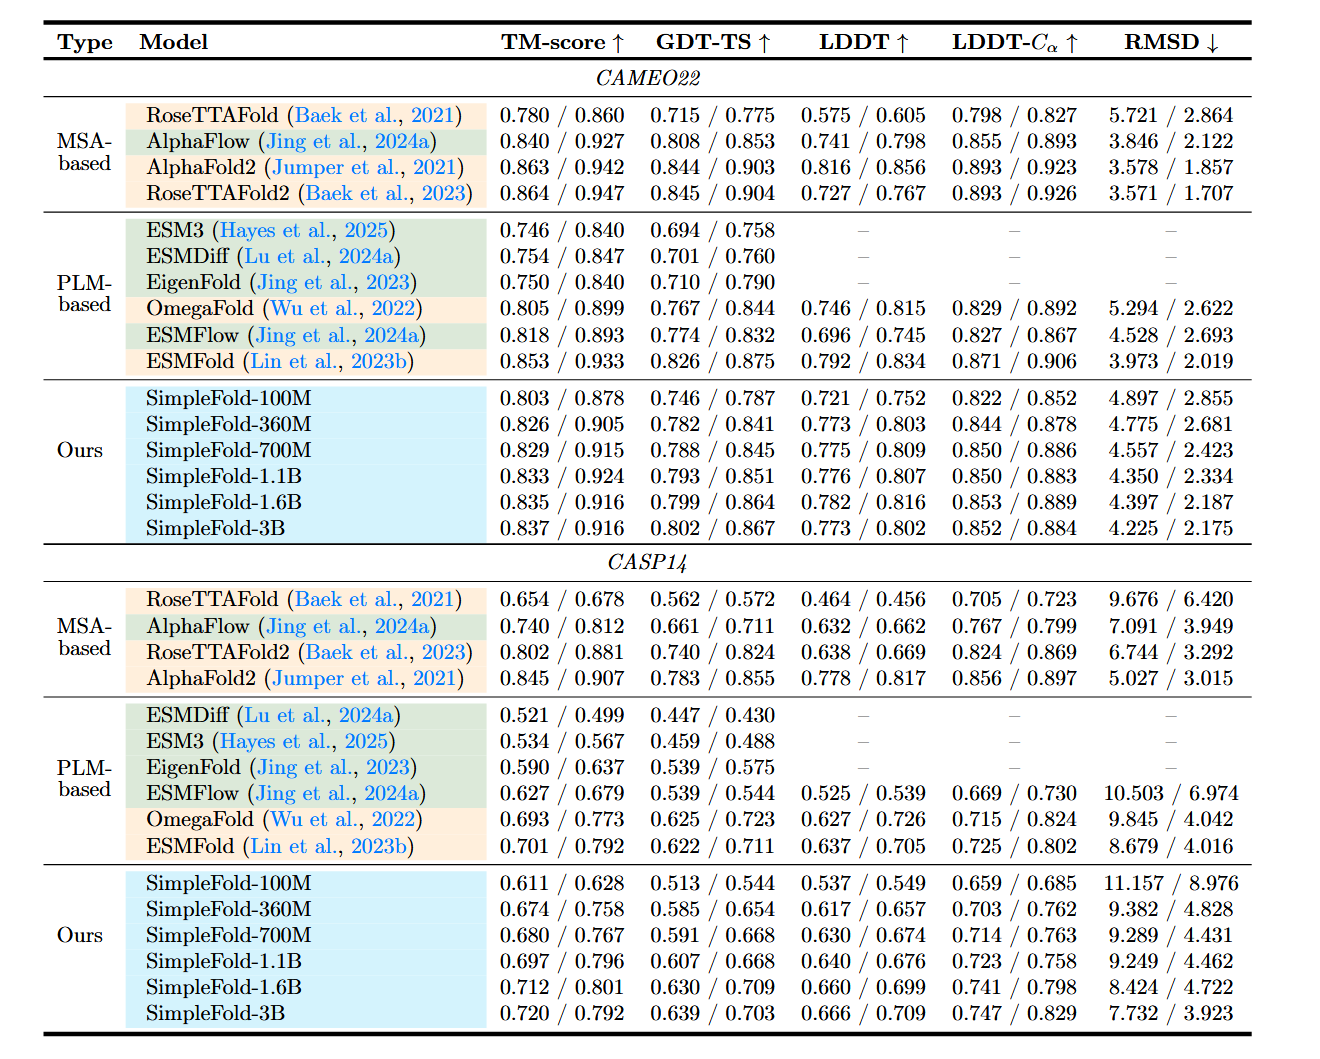
\includegraphics[width=0.5\textwidth]{../figures/simplefold2.png}
    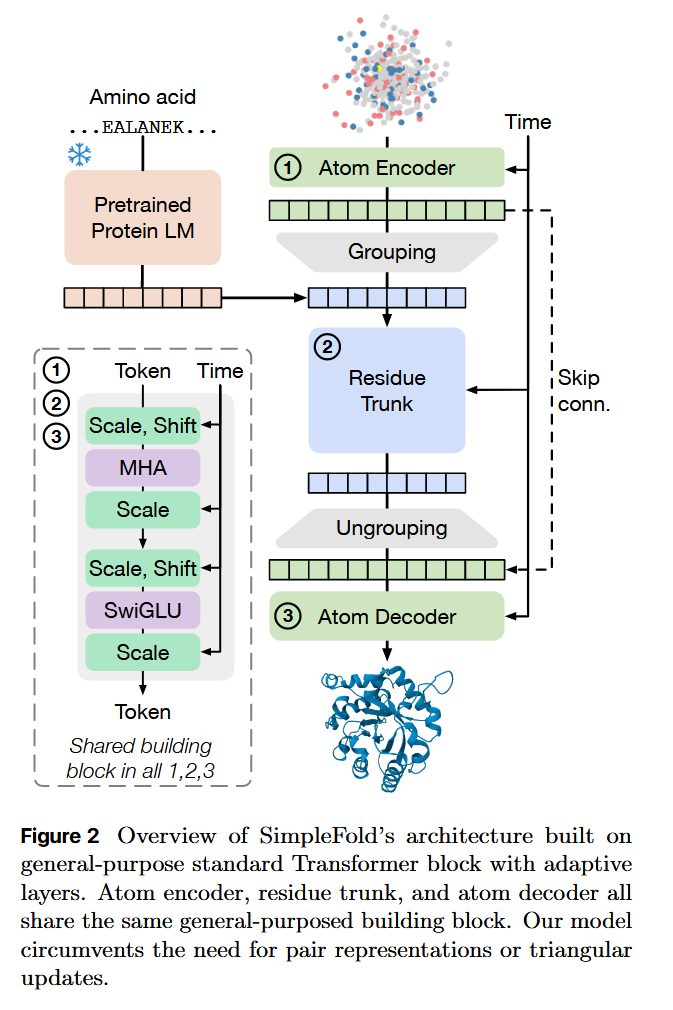
\includegraphics[width=0.3\textwidth]{../figures/simplefold3.png}
\end{figure}
\end{frame}


\begin{frame}{Results}
\begin{figure}
    \centering
    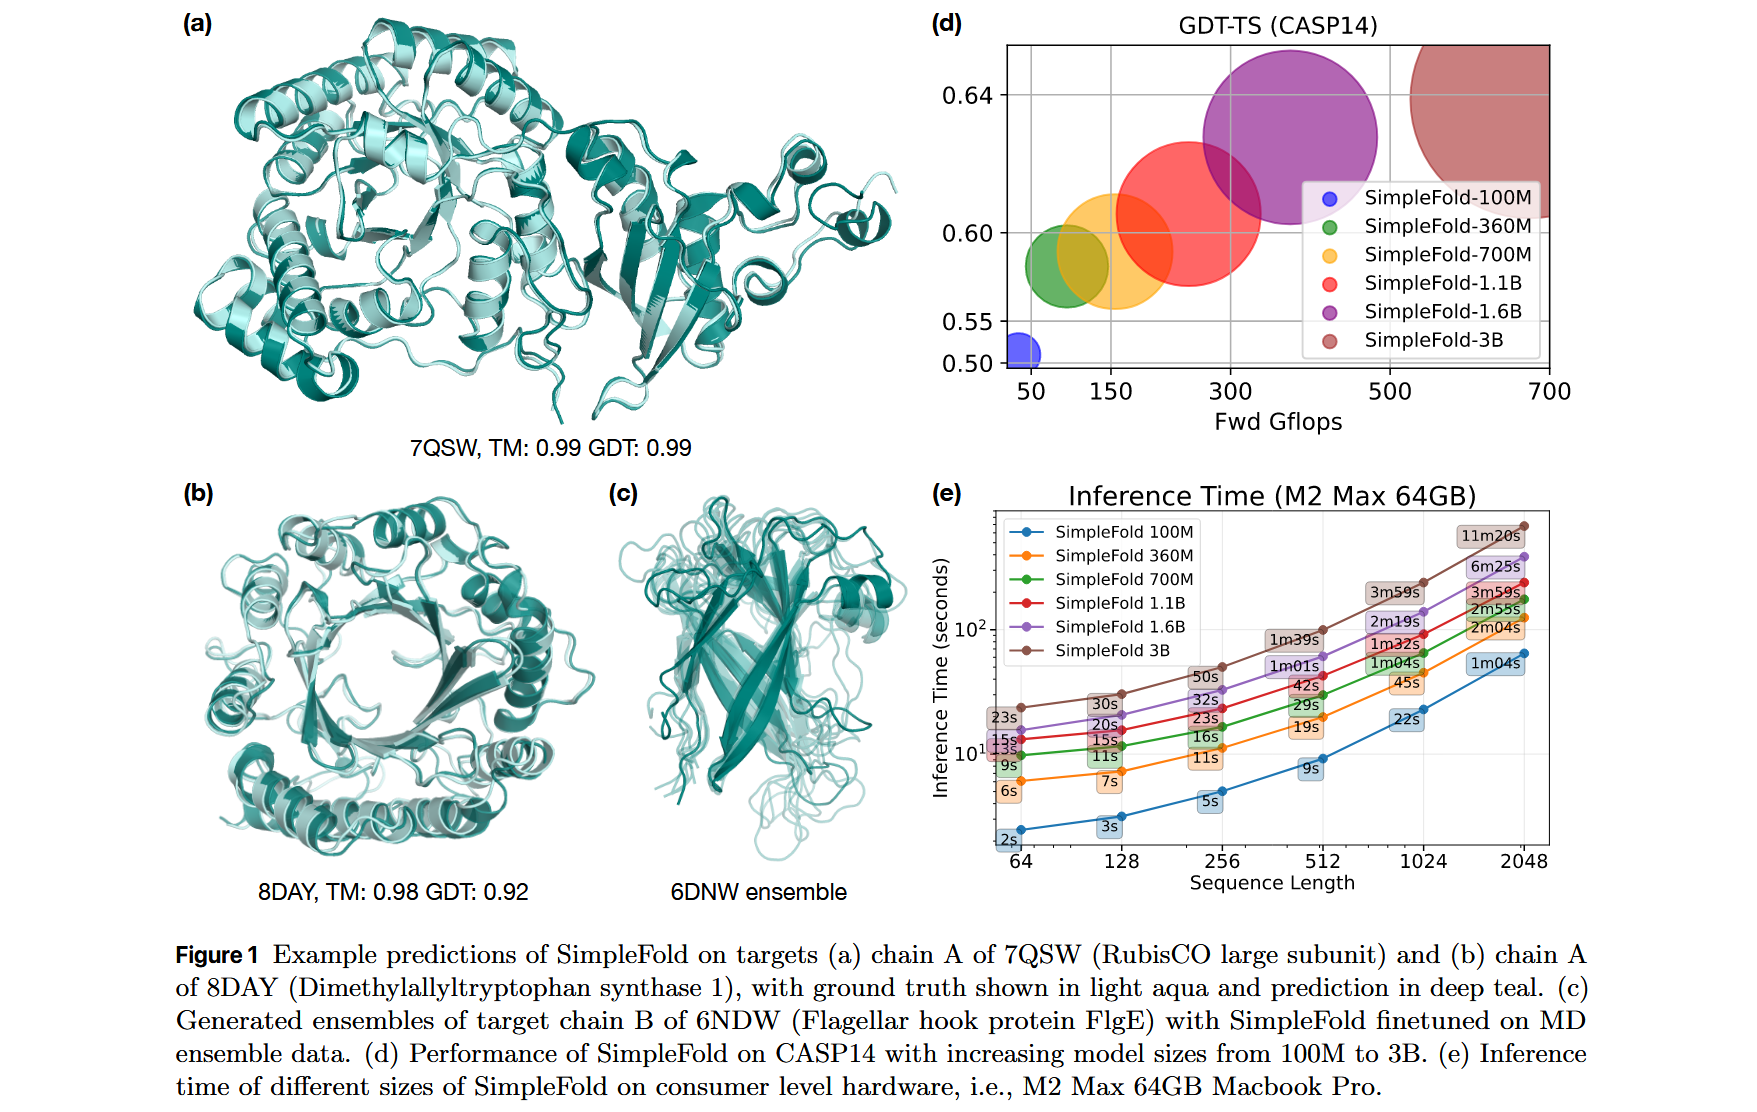
\includegraphics[width=0.75\textwidth]{../figures/simplefold1.png}
\end{figure}
\end{frame}

\begin{frame}{Scalability}
\begin{figure}
    \centering
    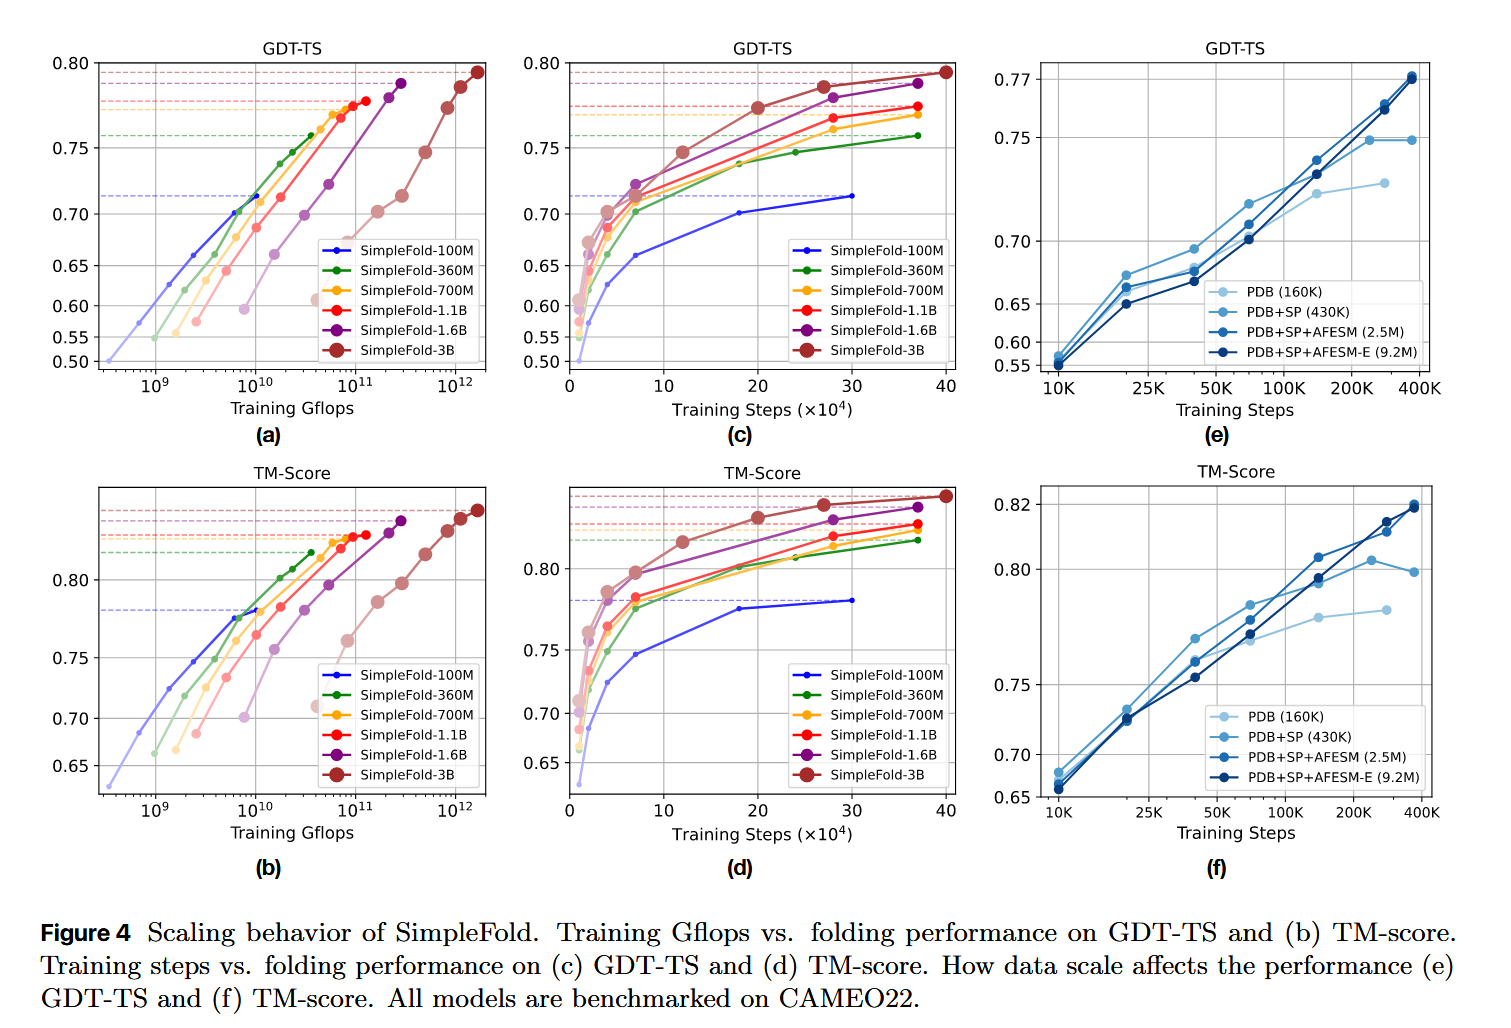
\includegraphics[width=0.65\textwidth]{../figures/simplefold4.png}
\end{figure}
\end{frame}

\subsection{AlphaFold 3}

\begin{frame}{AlphaFold 3}

See the pdfs.

\end{frame}


\subsection{UniGenX}
\begin{frame}{UniGenX}
See the MS PowerPoint presentation for more details.
\end{frame}

\subsection{RFDiffusion}

\subsection{MPNN}

\section{Conclusion}

\begin{frame}{Summary}
AI for Science represents a paradigm shift in how we approach scientific research:
\begin{itemize}
    \item \textbf{Acceleration}: Faster discovery and development cycles
    \item \textbf{Integration}: Combining data-driven and physics-based approaches
    \item \textbf{Automation}: Reducing manual work in scientific research
    \item \textbf{Insights}: Discovering patterns humans might miss
\end{itemize}
\end{frame}

\begin{frame}{The Future of AI for Science}
\begin{itemize}
    \item \textbf{Democratization}: Making advanced scientific tools accessible to all researchers
    \item \textbf{Interdisciplinary collaboration}: Breaking down silos between scientific fields
    \item \textbf{Scientific method evolution}: How AI changes the scientific process
    \item \textbf{Grand challenges}: Tackling humanity's biggest scientific problems
\end{itemize}
\end{frame}

\begin{frame}{Questions for Discussion}
\begin{enumerate}
    \item How can we ensure AI for Science maintains scientific rigor and reproducibility?
    \item What are the implications of AI for the future of scientific careers?
    \item How should we balance AI automation with human scientific intuition?
    \item What ethical guidelines should govern AI for Science research?
\end{enumerate}
\end{frame}

% Thank you slide  
\begin{frame}{Welcome inputs}  
  \centering  
  Any comments?
  \\[2em]
  Welcome your inputs!  
\end{frame}  
  
\end{document}  
